%!TEX root = ../main.tex

\chapter{Appendix A}

\label{AppendixA}

% Bisher: Daten -> metr. R�ume -> fuzzy simplicial sets
% Ziel:   Daten -> metr. R�ume -> VR complex

% Wenn VR Komplex ausreichend, betrachte nur 1-Skelet und berechne Homologie darauf.
% Siehe Oudot s.48, funktioniert noch nicht f�r Filtrationen. 

%----------------------------------------------------------------------------------------

% TODO: evtl Cech und VR in Grundlagen
\section{Homologie}
	% Hom�omorphismus, Homologie (Gruppen), homologie Equivalenz,
	Eine bekannte Aussage, welche der Topologie entstammt, ist, dass eine Kaffeetasse das Gleiche \textit{topologische Objekt} 
	wie ein Donut ist. Dies ist dadurch begr�ndet, dass man eine Kaffeetasse durch strecken und stauchen 
	(ohne rei�en) in einen Donut transformieren kann. Diese \textit{Gleichheit} l�sst sich wie folgt mathematisch darstellen:

	\begin{defn}[Stetige Abbildung]
		Sei ...
	\end{defn}

	\begin{defn}[Hom�omorphismus]
		Sei ...
	\end{defn}

	Nun werden wir den Begriff der Homologie einf�hren. Daf�r werden wir den Begriff der simplizialen Komplexe 
	ben�tigen um zuerst die simpliziale Homologie einzuf�hren.

	\begin{defn}[Simplizialer Komplex]
		Sei ...
	\end{defn}

	\begin{defn}[Abstrakter simplizialer Komplex]
		Sei ...
	\end{defn}

	\begin{ex}
		\cech-Komplex
	\end{ex}

	\begin{ex}
		VR-Komplex
	\end{ex}

	\begin{defn}[Homologie]
		Sei ...
	\end{defn}

	\begin{defn}[Homologiegruppe]
		Sei ...
	\end{defn}

	\begin{ex}
		Die Homologiegruppen eines Balls, Donuts, Graphen, ...
	\end{ex}

	\begin{defn}[Filtration]
		Sei $T \subseteq \R$, eine \textit{Filtration} $\mathcal{X}$ �ber $T$ ist eine Familie von 
		topologischen R�umen $\{X_i\}_{i \in T}$, so dass $X_i \subseteq X_j$ 
		f�r $i \leq j \in T$.  % (Oudot s.29)
	\end{defn}

	\begin{rem}
		Eine Filtration $\mathcal{X}$ wird meist nicht als Familie verschiedener topologischer 
		R�ume $X_i$ angesehen, sondern als ein einziger Raum, welcher sich im Laufe der Zeit 
		\enquote{transformiert}. Siehe dazu \cite{Oudot}.  % (Oudot s.30)
		Dies stimmt mit unserem Bild �berein, den $\epsilon$-Parameter eines \cech-Komplexes %TODO: Satz l�schen und motivation cech komplex nennen
		immer gr��er werden zu lassen. Wir werden \textit{persistente Homologie} nutzen um 
		die homologischen Eigenschaften zu beschreiben, welche f�r alle $i \in T$ erhalten 
		(bzw. persistent) bleiben.
	\end{rem}

	% TODO: Oudot Kap. 4,5 f�r Anwendungen von persistenter Homologie

	% TODO: Bemerkung, dass \mathcal{X} eine Repr�sentation eines Poset ist (siehe Oudot s.29)

	\begin{ex}
		% TODO: warum?
		Insbesondere ist somit der \cech-Komplex eine Filtration, da ...
	\end{ex}

	\begin{ex}
		% TODO: warum?
		Eine weitere Filtration ist der Vietoris-Rips-Komplex
	\end{ex}

	\begin{rem} % TODO: Bem in Def umwandeln
		Der VR-Komplex ist ein Beispiel eines Clique-Komplexes und wird als solcher 
		eindeutig durch sein 1-Skelet identifiziert. Sei $V$ ein VR-Komplex und $V^1$ das 
		zugeh�rige 1-Skelet. Dann erh�lt man $V$ aus $V^1$, indem man alle Cliquen im 
		$V^1$ zugrundeliegenden Graphen bestimmt. Eine k-Clique ist ein vollst�ndiger Subgraph 
		mit k Knoten. 
	\end{rem}

	Es gibt weitere Formen von Komplexen, die bekanntesten sind die CW-Komplexe und Zellkomplexe. 
	Ziel ist es stets mit Hilfe einfacher Konstrukte die Topologie eines Raums zu beschreiben.

	Die vom \cech-Komplex und vom Vietoris-Rips-Komplex beschriebene Homologie kann sich unterscheiden (siehe Abbildung \ref{fig:Cech_VR}).

	\begin{figure}
		%\centering
		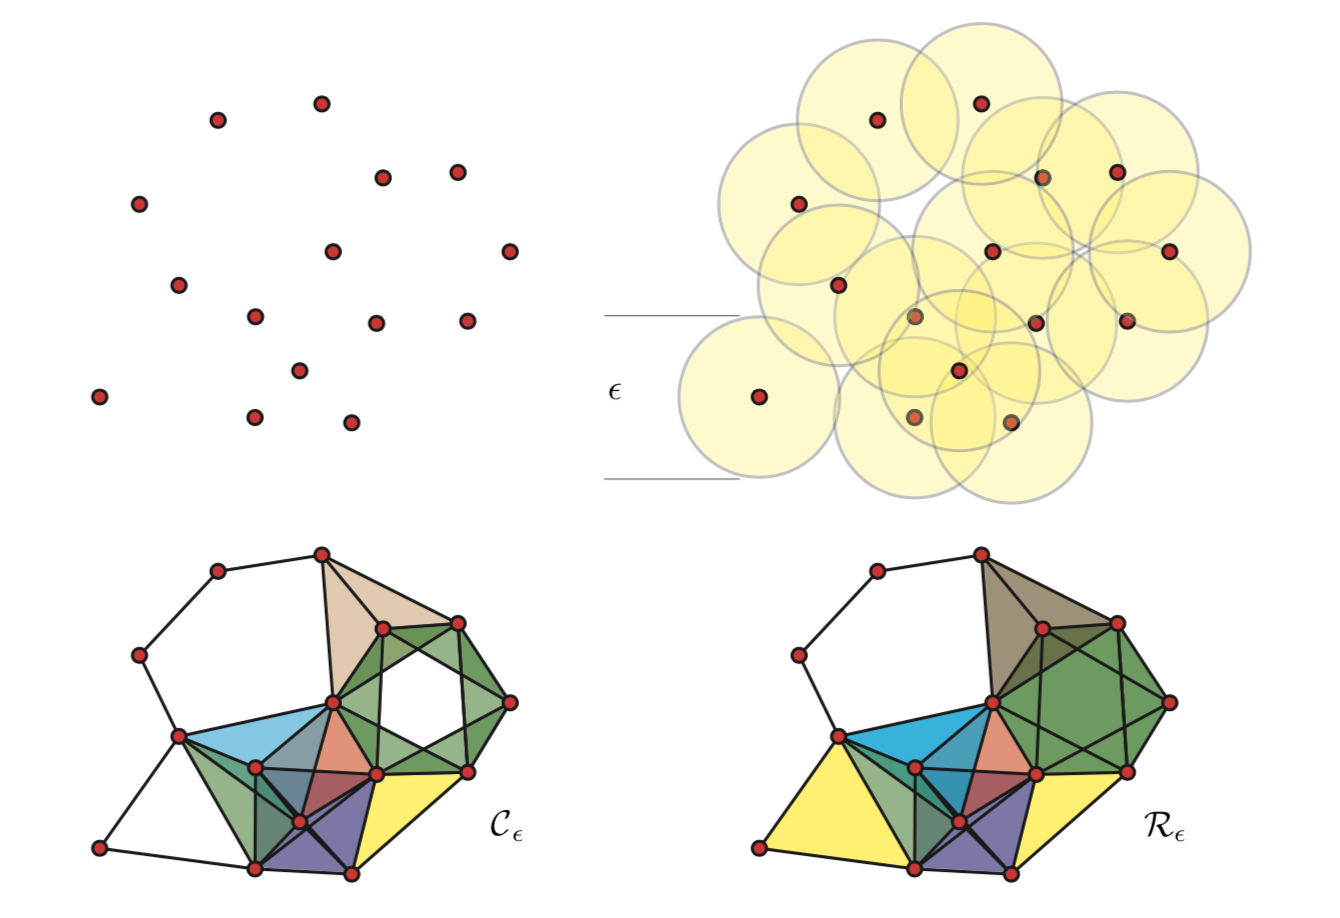
\includegraphics[width=400px, height=274px]{Figures/Cech_VR_complex}  % width=1\textwidth
		%\decoRule
		\captionsetup{justification=RaggedRight}  % centerfirst
		\caption[Versch. Komplexe]{Eine Punktwolke [oben links] kann zu einem \cech-Komplex [unten links] 
								   oder einem VR-Komplex [unten rechts] basierend auf dem Parameter $\epsilon$ 
								   konstruiert werden. Die Homotopietypen der $\epsilon/2$ �berdeckung vom 
								   \cech-Komplex ($S^1 \vee S^1 \vee S^1$), w�hrend das VR-Komplex die Homotopietypen 
								   ($S^1 \vee S^2$) besitzt. (\textit{Quelle:} \cite{Barcodes})}

		\label{fig:Cech_VR}
	\end{figure}

	Wir ben�tigen nun noch den Begriff einer \textit{guten �berdeckung} um dann eine geeignete Aussage �ber einen \cech-Komplex einer Menge zu machen. 

	\begin{defn}[�berdeckung]
		Eine �berdeckung eines topologischen Raumes ist \dots
		Eine gute �berdeckung ist \dots
	\end{defn}

	\begin{NT}  % Nerv Theorem
		% Ein top. Raum ist homotopie equivalent zu einer endlichen guten �berdeckung. 
		Sei ...
		\label{thm:NT}
	\end{NT}
	
	Das Nerv Theorem \ref{thm:NT} liefert uns eine Aussage dar�ber, dass ein topologischer Raum $X$ zu einer endlichen guten 
	�berdeckung von $X$ homotopie�quivalent ist.
	Wie wir sehen ist die Konstruktion stark abh�ngig vom $\epsilon$-Parameter. Um dem 
	entgegenzuwirken nutzt man die Idee der \textit{persistenten Homologie}. Dabei 
	wird betrachtet wie sich die Homologie eines Raumes f�r eine monoton wachsende Folge 
	$(\epsilon_i)_{i \in \N}$ verh�lt.

	F�r den von uns betrachteten Fall, die Struktur einer Riemannschen Mannigfaltigkeit $(\M, g)$ zu beschreiben, werden wir 
	Annehmen, dass die Daten $\mathbf{x}_i \in X$ gleichverteilt bez�glich der Riemannmetrik $g$ sind, bzw. $g$ so w�hlen, das 
	die Annahme erf�llt ist. Somit erhalten wir eine gute �berdeckung ohne eine Abh�ngigkeit von $\epsilon$ zu haben. 
